%%%%%%%%%%%%%%%%%%%%%%%%%%%%%%%%%%%%%%%%%%%%%%%%%%%%%%%%%%%%%%%%%%%%%%%%%%%%%%%%
%2345678901234567890123456789012345678901234567890123456789012345678901234567890
%        1         2         3         4         5         6         7         8

\documentclass[letterpaper, 10 pt, conference]{ieeeconf}
\usepackage{graphicx}
\usepackage{amsmath}
\usepackage{gensymb}
\usepackage{relsize}
\usepackage{amsfonts}
\usepackage{mathtools}
\usepackage{lineno,amssymb,subcaption,algpseudocode,algorithm}
\usepackage[font={small}]{caption}
\usepackage{picins}
\usepackage{cleveref}
\usepackage{array}
\usepackage{float}
\usepackage{xcolor}

% Commands
\newcommand{\ubar}[1]{\text{\b{$#1$}}}
\DeclareMathOperator*{\minimize}{minimize}
\DeclareMathOperator*{\argmin}{argmin}
\DeclareMathOperator*{\subj}{subject\;to}
\DeclareMathOperator*{\st}{s.t.}

\newcommand{\cx}{\textsf{x}}
\newcommand{\cz}{\textsf{z}}
\newcommand{\cl}{\lambda}
\newcommand{\J}{\textsf{J}}
\newcommand{\cf}{\textsf{f}}
\newcommand{\cg}{\textsf{g}}
\newcommand{\ch}{\textsf{h}}
\newcommand{\X}{\textsf{X}}

\newlength\figwidth
\setlength\figwidth{\columnwidth}
\newlength\figheight
\setlength\figheight{5cm}
\newcolumntype{P}[1]{>{\centering\arraybackslash}p{#1}}


\bibliographystyle{ieeetr}

%\documentclass[a4paper, 10pt, conference]{ieeeconf}      % Use this line for a4 paper

\IEEEoverridecommandlockouts                              % This command is only needed if
                                                          % you want to use the \thanks command

\overrideIEEEmargins                                      % Needed to meet printer requirements.

% See the \addtolength command later in the file to balance the column lengths
% on the last page of the document

% The following packages can be found on http:\\www.ctan.org
%\usepackage{graphics} % for pdf, bitmapped graphics files
%\usepackage{epsfig} % for postscript graphics files
%\usepackage{mathptmx} % assumes new font selection scheme installed
%\usepackage{times} % assumes new font selection scheme installed
%\usepackage{amsmath} % assumes amsmath package installed
%\usepackage{amssymb}  % assumes amsmath package installed

\title{\LARGE \bf
Distributed model predictive control of multiple
vehicles transporting a flexible payload*
}


\author{Sampath Kumar Mulagaleti$^{2}$, Ruben Van Parys$^{1}$ and Goele Pipeleers$^{1}$%  <-this % stops a space
\thanks{*This work benefits from KU Leuven-BOF PFV/10/002 Centre of Excellence: Optimization in Engineering (OPTEC); from the project G0C4515N of the Research Foundation-Flanders (FWO-Flanders); and from the KU Leuven Research project C14/15/067: B-spline based certificates of positivity with applications in engineering. Ruben Van Parys is a PhD fellow of FWO-Flanders. Flanders Make is the Flemish strategic research centre for the manufacturing industry. }%
\thanks{$^{1}$The authors are with the MECO Research Team, Department Mechanical Engineering, KU Leuven and with the DMMS lab, Flanders Make, Leuven, Belgium. $^{2}$The author is with the IMT School for Advanced Studies Lucca, 55100, Italy. Email:
	 \texttt{s.mulagaleti@imtlucca.it}}
}

\begin{document}



\maketitle
\thispagestyle{empty}
\pagestyle{empty}


%%%%%%%%%%%%%%%%%%%%%%%%%%%%%%%%%%%%%%%%%%%%%%%%%%%%%%%%%%%%%%%%%%%%%%%%%%%%%%%%
\begin{abstract}
This paper presents a control strategy for multiple vehicles that cooperatively transport a flexible payload. To this end, an algorithm is developed which generates optimal trajectories for the vehicles to follow. Solving an optimization problem composes the core of the algorithm. The problem is first decomposed over the vehicles using the Alternating Direction Method of Multipliers (ADMM) algorithm. This results in each vehicle solving a sub-problem to generate its own optimal trajectory. The algorithm instructs that the optimization problem be solved repeatedly in a receding horizon fashion, making it fit into a distributed model predictive control (DMPC) framework. One ADMM iteration is performed per DMPC iteration, reducing the inter-agent communication rate. Numerical validation of the developed control scheme is performed and the results are presented.
\end{abstract}


%%%%%%%%%%%%%%%%%%%%%%%%%%%%%%%%%%%%%%%%%%%%%%%%%%%%%%%%%%%%%%%%%%%%%%%%%%%%%%%%
\section{INTRODUCTION}

Payload transportation tasks are ubiquitous in industrial environments. These payloads can vary greatly in weights, necessitating multiple transportation solutions of different payload capacities within the same logistics structure. An alternative to this would be to use multiple vehicles to cooperatively tow a payload, with the number of vehicles chosen according to the towing requirements. To enable such a multi-agent system to work autonomously and transport the payload to a desired location, control strategies are required which perform coordinated motion of the vehicles.
\\
\indent Transportation of objects with multiple vehicles is a standard problem in robotics and control. Some of the early approaches to model and control such systems are presented in \cite{c1,c2,c3}, and an optimal control approach in \cite{c4}. More recent approaches are formulated in a Model Predictive Control (MPC) framework, which allows to explicitly incorporate system constraints in the optimization problem. Such techniques have been applied to perform trajectory tracking with multiple vehicles moving in a desired formation \cite{c5}. Motion planning for multiple vehicles moving in a formation is done within a receding horizon framework in \cite{c6}, utilizing a leader-follower strategy. Such a strategy is not robust against possible failure of the leader agent. This necessitates development of strategies in which each agent performs an equivalent task within the multi-agent system. This leads to the domain of Distributed Model Predictive Control (DMPC). Within the DMPC framework, the control problem is distributed over the agents. Since an optimization problem underlies the MPC framework, DMPC based techniques usually employ distributed optimization methods to distribute the optimization problem over the agents \cite{c7}. Motion planning algorithms are designed within this framework in \cite{c8} and \cite{c16} for formation control of multiple agents.
\\
\indent
Unlike formation control problems, agents in payload transportation problems are dynamically coupled. This means that a change in state of one of the agents alters the state of the others. The coupled dynamics act as constraints shared by all the agents within the multi-agent system, and decomposing the centralized problem for DMPC purposes would require decomposing the coupling dynamics constraint. Decoupling of dynamics is done using primal decomposition
 in \cite{c10}, in which, linear systems are considered, and an optimal consensus problem is solved. In optimal consensus problems, multiple optimization variables are driven to the
 same value over iterations. Another approach based on dual decomposition, is discussed in \cite{c11}. In this work, the variable splitting method of \cite{c8} is employed. According to this method, copies of states of a multi-agent system that are not local to a constituent vehicle are introduced as exogenous inputs on the vehicle. More robust methods based on the ADMM are formulated in \cite{c12}, which consider coupled objective functions in addition to coupled nonlinear dynamics. Another alternative is introduced in \cite{c13}, where the
 ADMM-consensus problem introduced in \cite{c14} is combined with the idea of introducing copies of neighboring states from \cite{c11}.
 \\
 \indent
 This work extends the DMPC scheme introduced for the formation control problem in \cite{c16}, to the cooperative payload transportation problem. The main advantage of this scheme is that it achieves a decentralized-consensus in a dynamically coupled system, by decoupling the 2nd ADMM step using a novel variable-copying scheme. In order to reduce the communication and computation load, 1 ADMM iteration is performed per DMPC iteration, and the ADMM iterations are supported by inter-vehicle communication. The proposed scheme is implemented using a spline-based parameterization discussed in \cite{c16}, and a numerical validation of the algorithm is performed.
\\ \indent
Section  II  introduces  the  motion  planning  problem  for
cooperative payload transportation problem, and Section III describes how
this  problem is solved in an online distributed manner. Results from simulations based on the proposed approach are presented in Section IV, and the conclusions in Section V.
\section{PROBLEM FORMULATION}
\subsection{System model}
The dynamic system under consideration here is shown in Figure \ref{2D_schematic}. It is modeled as multiple holonomic vehicles attached through 1D spring-damper elements to a common payload. The payload and the holonomic vehicles are abstracted as point masses, and are constrained to move in a 2D plane. Dynamic spring-mass-damper models are used to describe the system in the optimization problem. Coulomb friction is ignored in the model. The free length of the flexible elements is assumed to be $0$ m, resulting in the vehicles only applying a pulling force on the payload. In this paper, $N$=3 vehicles are considered. 

\begin{figure}
  \centering
  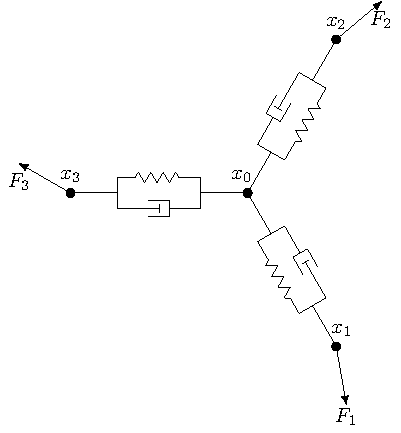
\includegraphics[scale=0.6]{figures/schematic.pdf}
  \caption{Dynamic model decoupling}
  \label{2D_schematic}
\end{figure}

\subsection{Optimal control problem}
This section discusses the formulation of the considered optimal control problem. The optimization variables are the payload and the vehicle trajectories. The solution of this problem are the trajectories that transport the payload to a location closest to its goal $x_d \in \mathbb{R}^2$ within the time horizon $T$ over which the problem is solved.
The payload trajectory is represented by the vector ${x_0:[0,T] \rightarrow \mathbb{R}^2}$ and that of each vehicle $i$ by ${x_i:[0,T] \rightarrow \mathbb{R}^2}$.
 The formulation is shown in \eqref{label:central}.
\begin{equation}
  \label{label:central}
  \begin{aligned}
    & \minimize_{x_0(.),x_1(.),x_2(.),x_3(.)} \qquad \mathlarger{\int_0^T} \mathlarger{||}x_0(t)-x_d\mathlarger{||}_1 dt \\
    & \qquad \subj
     \qquad \text{  } g(x_0(t),x_1(t),x_2(t),x_3(t)) = 0 \\
    &	\qquad  \qquad \qquad \quad \quad \quad h_{ij}(x_0(t),x_i(t),x_j(t)) \leq 0 \\
    &	\qquad  \qquad \qquad \quad \quad \quad \ubar{l} \preceq f_i(x_0(t),x_i(t)) \preceq \bar{l}\\
    &	\qquad  \qquad \qquad \quad \quad \quad \ubar{d} \preceq d_i(x_i(t)) \preceq \bar{d} \\
    &	\qquad  \qquad \qquad \quad \quad \quad \{x_0^{(k)}(0), x_0^{(k)}(T)\}  = X^p \\
      &	\qquad  \qquad \qquad \quad \quad \quad \{x_i^{(k)}(0), x_i^{(k)}(T)\}  = X^i \\
    &	 \qquad \qquad \qquad \quad \quad \quad \forall t \in [0,T], \quad \forall i,j \in \{1,2,3\}, i \neq j
  \end{aligned}
\end{equation}
As mentioned earlier, the coupled payload dynamics of the multi-agent system are modeled as constraints in the optimization problem. It is expressed in \eqref{g}. The time dependence of the trajectories is dropped for ease of notation. The parameters $m_i$ and $m_0$ represent vehicle $i$'s and payload's mass respectively, and $c_i$ and $k_i$ represent damping and stiffness coefficients of flexible element $i$.
\begin{equation}\label{g}
\begin{aligned}
g(x_0,x_1,x_2,x_3) &= m_0\ddot{x}_0 +  \mathlarger{\sum\limits_{i=1}^{3}}
\begin{bmatrix}{c_i(\dot{x}_i-\dot{x}_0) + k_i(x_i - x_0)} \end{bmatrix}\\
\end{aligned}
\end{equation}
\noindent
Intra-vehicle collisions are avoided by the function $h_{ij}$, expressed in \eqref{h}, utilizing the inner-product notation. It limits the angles between the vehicles to lie at greater than 90$\degree$ when subtended at the payload. Unlike the complete coupled constraint $g$, this is a constraint involving nearest neighbors.
 \begin{equation}\label{h}
\begin{aligned}
h_{ij}(x_0,x_i,x_j) &= \mathlarger{\langle} x_i - x_0,x_j - x_0 \mathlarger{\rangle}
\end{aligned}
\end{equation}
The function $f_i$ consists of individual vehicle $i$'s dynamics, and flexible element $i$'s length. The lower and upper bounds on these quantities are captured in vectors $\ubar{l}$ and $\bar{l}$ respectively. This function is shown in \eqref{f}.
 \begin{equation}\label{f}
 \begin{aligned}
 f_i(x_0,x_i) &=
 \begin{bmatrix}
   m_i\ddot{x}_i + c_i(\dot{x}_i-\dot{x}_0) + k_i(x_i-x_0) \\
  \mathlarger{\langle} x_i - x_0,x_i - x_0 \mathlarger{\rangle}
 \end{bmatrix} \\
 \end{aligned}
 \end{equation}
 Limitations on vehicle velocities and accelerations are expressed through the function $d_i$ shown in \eqref{d}, with the limits on these quantities captured in the vectors $\ubar{d}$ and $\bar{d}$.
 \begin{equation}\label{d}
 \begin{aligned}
 d_i(x_i) &=
 \begin{bmatrix}
  \dot{x_i}^T & \ddot{x_i}^T
 \end{bmatrix}^T \\
 \end{aligned}
 \end{equation}
 The remaining constraints represent limits on vehicle velocities and accelerations, and initial and final conditions on the vehicle and payload position trajectories and higher derivatives.
\section{Solution strategy}
\subsection{Spline parameterization}
Problem \eqref{label:central} represents an infinite dimensional problem, since the optimization variables $x_0(.)$ and $x_i(.)$ are infinite dimensional, and enforcing the constraints at all time results in an infinite number of constraints. In order to make the problem numerically tractable, a B-spline based parameterization of the optimization variables is used, along the lines of \cite{c15}. The continuous optimization variables are hence represented as linear combinations of piecewise polynomial B-spline basis functions $b_k(t)$, as expressed in \eqref{spline}.

\begin{equation}\label{spline}
x_i(t) = \mathlarger{\sum\limits_{k=1}^{n}} \cx_{i,k}b_k(t) = \cx_i^Tb(t) \quad \forall i \in \{0,1,.,N\}
\end{equation}

 The trajectories of each vehicle $i$ are consequently represented by the coefficient set $\cx_i$$=$ $\{\cx_{i,k}\}_{k=1}^{n}$ and those of the payload by $\cx_0$$=$$\{\cx_{0,k}\}_{k=1}^{n}$, for a chosen B-spline basis functions vector $b = [b_1,\ldots,b_n]^T$. Substituting these parameterizations in \eqref{label:central} results in an optimization problem with finite number of variables. A B-spline parameterization is chosen because of its convex hull property \cite{c15}, which dictates that the resultant spline function lies within the convex hull of the coefficients. Hence, the constraints on an infinite dimensional spline can be imposed on its coefficients, resulting in a finite number of constraints. Reducing potential conservatism is discussed in \cite{ms-6-163-2015}. Since the constraint functions $f_i$, $g$ and $h_{ij}$ are composed of polynomial combinations of the splines $x_i(t)$ and $x_0(t)$ and their derivatives, the resultant functions are splines in a B-spline polynomial basis as well. The coefficients of these splines are polynomial combinations of $\cx_0$ and $\cx_i$. Following the convex hull property, these constraints are transformed to $\cf_i$, $\cg$ and $\ch_{ij}$ respectively. The coefficients, and functions composed of those coefficients are indicated in a sans-serif font. Non-coupled constraints on the spline coefficients are captured in $\X_i$ and $\X_0$.
The resulting formulation is seen in \eqref{withparam}.

 \begin{equation}
   \label{withparam}
   \begin{aligned}
     & \minimize_{\forall i:\cx_i,\cx_0} &&  \J(\cx_0) \\
     & \subj
     &      & \cg(\cx_0,\cx_1,\cx_2,\cx_3) = 0 \\
     &        && \ch_{ij}(\cx_0,\cx_i,\cx_j) \leq 0 \\
     &	&& \ubar{l} \preceq \cf_i(\cx_0,\cx_i) \preceq \bar{l}\\
     &        && \cx_i \in \X_i \\
     &        && \cx_0 \in \X_0 \\
     &                                && \forall i,j \in \{1,2,3\}, i \neq j
   \end{aligned}
 \end{equation}
 The MPC updating scheme proposed in \cite{c16} for optimization variables expressed in a B-spline basis can be used on a centralized processor, provided it has access to all $\cx_i$ and $\cx_0$ variables. This scheme is summarized in Algorithm~\ref{alg:mpc}. The vehicle and payload positions that are estimated at time $(k+1)\Delta T$ are incorporated into the feasible sets $\X_i$ and $\X_0$ while solving the problem for $\cx_i^{k+1}$ and $\cx_0^{k+1}$. The hot-start coefficients are $\tilde{\cx}_i^k$ and $\tilde{\cx}_0^k$ are obtained by expressing $\cx_i^k$ and $\cx_0^k$ in current MPC horizon's basis, as discussed in \cite{c16}.

 \algblockdefx[Name]{Repeat}{Until}[1][Unknown]{\textbf{Repeat} #1}{\textbf{Until }}
 \begin{algorithm}[t]
 \caption{Spline-based MPC}\label{alg:mpc}
 \begin{algorithmic}[1]
 \Repeat[every $\Delta T$:  $k=0,1,\ldots$]
   \State Extract $x_i^k(t)$ from $\cx_i^k$ for each Vehicle $i$.
   \State Vehicle $i$ starts following trajectory $x_i^k(t)$
   \State Estimate $\hat{x}_i^k$ and $\hat{x}_0^k$ at time $(k+1)\Delta T$
   \State Compute $\tilde{\cx}_i^k$ and $\tilde{\cx}_0^k$ over the updated horizon.
   \State Compute $\cx_i^{k+1}$ and $\cx_0^{k+1}$ by solving \eqref{withparam}, using $\hat{x}_i^k$, $\hat{x}_0^k$ as initial conditions and $\tilde{\cx}_i^k$ as hot start coefficients
 \Until target reached
 \end{algorithmic}
 \end{algorithm}

 \subsection{Distributed formulation}
 The purpose of this section is to split the optimization problem \eqref{withparam} into 3 separate problems, one for each vehicle. This allows each vehicle to solve for its own trajectory, aided by communication between the vehicles. The first step is the introduction of copies of the payload variables $\cx_0$ on each vehicle, represented by $\cx_{i0}$. This substitution results in 3 copies of the payload dynamics constraint $\cg$, each one being $\cg(\cx_{i0},\cx_i,\cx_j) = 0$, where $\cx_j = \{\cx_1,\cx_2,\cx_3\}\ominus \cx_i$. The symbol $\ominus$ denotes the set-difference operator.
 \\ \indent
 The payload dynamics constraint is further decoupled by borrowing ideas from \cite{c11}, which dictates that the variables $x_{j}(t)$ of vehicle $j$ which affect the dynamics of vehicle $i$ can be modeled as exogenous inputs $x_{ij}(t)$ acting on vehicle $i$. The new variables $x_{ij}(t)$ are hence local to vehicle $i$, and are parameterized by the spline coefficients $\cx_{ij}$. The payload dynamics constraint is thus further modified as $\cg(\cx_{i0},\cx_i,\cx_{ij}) = 0$. This is supported by consensus constraints between  $\cx_{j}$ and $\cx_{ij}$. Similar substitutions are performed in the anti-collision constraints $\ch_{ij}$. Following a modification of the consensus constraints presented in \cite{c16}, consensus variables $\cz_{ij}$ are introduced on each vehicle $i$, which act as a balance between $\cx_{j}$ and $\cx_{ij}$. The modified optimization problem with local copy variables, consensus variables, and consensus constraints is shown in \eqref{main_problem}.
   \begin{equation}
     \label{main_problem}
     \begin{aligned}
       & \minimize_{\forall i,j,i \neq j:\cx_i,\cx_{ij},\cz_{ij},\cx_{i0}} &&  \sum\limits_{i=1}^{3}\J(\cx_{i0}) \\
       & \subj
       && \ubar{l} \preceq \cf_i(\cx_{i0},\cx_i) \preceq \bar{l}\\
       &       && \cg(\cx_{i0},\cx_i,\cx_{ij}) = 0 \\
       &        && \ch_{ij}(\cx_{i0},\cx_i,\cx_{ij}) \leq 0 \\
       &         && \cx_{ij} = \cz_{ij},\, \cx_{j} = \cz_{ij} \\
       &        && \cx_i \in \X_i,\, \cx_{i0} \in \X_0 \\
       &                                && \forall i,j \in \{1,2,3\}, i \neq j
     \end{aligned}
   \end{equation}

  \indent
 The optimization problem \eqref{main_problem} can now be decoupled using the Alternating Direction Method of Multipliers (ADMM). The ADMM algorithm solves the dual of \eqref{main_problem}, after augumenting it with a quadratic term to improve convergence properties. To minimize the duality gap, the fewest number of constraints are dualized according to \cite{c8}. Hence, only the consensus equality constraints are moved into the objective function to form the Lagrangian: \vspace{-20pt} \\

 \begin{equation}\label{Lagrangian}
   \begin{aligned}
   \mathcal{L}_\rho &=
  {\mathlarger{\sum\limits_{i=1}^{3}}}
  {\mathlarger{\mathlarger{(}}}\J_i(\cx_{i0}) +
 \mathlarger{\sum\limits_{j \neq i}} \mathlarger{(} \lambda_{ij}^T(\cx_{ij} - \cz_{ij}) + \cfrac{\rho}{2} \mathlarger{||}\cx_{ij} - \cz_{ij}\mathlarger{||}_2^2{{\mathlarger{)}}} \\ & \qquad \qquad \qquad
  + \mathlarger{\sum\limits_{j \neq i}} \mathlarger{(} \mu_{ij}^T(\cx_{j} - \cz_{ij}) +
   \cfrac{\rho}{2} \mathlarger{||}\cx_{j} - \cz_{ij}\mathlarger{||}_2^2 \mathlarger{)}\mathlarger{\mathlarger{\mathlarger{)}}}
   \vspace{-10pt} \\
   &= {\mathlarger{\sum\limits_{i=1}^{3}}}  \mathcal{L}_{\rho,i} (\cx_{i0},\cx_{ij},\cz_{ij},\lambda_{ij},\cx_{j},\cz_{ij},\mu_{ij}) \\
   &= {\mathlarger{\sum\limits_{i=1}^{3}}}  \mathcal{L}_{\rho,i} (\cx_{i0},\cx_{ij},\cz_{ij},\lambda_{ij},\cx_{i},\cz_{ji},\mu_{ji})
   \end{aligned}
   \end{equation}
The dual variables introduced in the Lagrangian formulation corresponding to the equality constraints are $\lambda_{ij}$ and $\mu_{ij}$. The last equality in \eqref{Lagrangian} is valid due to the bidirectionality of interaction amongst the vehicles: variables on vehicle $i$ affecting the dynamics of vehicle $j$ correspond to the variables on vehicle $j$ affecting dynamics of vehicle $i$.
Since the constraints are now completely decoupled, the feasible set on each vehicle $i$ is represented by $\{\cx_{i},\cx_{i0},\cx_{ij}\} \in \Phi_i$. The dual function of \eqref{main_problem} is shown in \eqref{dual_problem}.
\begin{equation}\label{dual_problem}
q(\lambda_{ij},\mu_{ij}) = \inf_{\substack{\{\cx_{i},\cx_{i0},\cx_{ij}\} \in \Phi_i \\ \forall i,j \in \{1,2,3\}, i \neq j}} \mathcal{L}_{\rho}\
\end{equation}

The dual variables are found by maximizing the dual function $q$ with respect to the lagrangian multipliers. The maximization is performed through gradient ascent in the ADMM algorithm. For this, the primal variables $\cx_{ij}^k$,$\cx_{j}^k$ and $\cz_{ij}^k$ from iteration $k$ are updated in iteration $k+1$, and the gradient of the dual function $q$ is calculated in the directions of the lagrangian multipliers according to \eqref{gradients}.
\begin{equation}\label{gradients}
  \begin{aligned}
    \nabla_{\lambda_{ij}} q    &= \cx_{ij}^{k+1} - \cz_{ij}^{k+1}\\
    \nabla_{\mu_{ij}} q &= \cx_{j}^{k+1} - \cz_{ij}^{k+1}
  \end{aligned}
\end{equation}
 An optimal step of length $\rho$ in these directions is taken. The primal variables are updated in two steps in a Gauss-Seidel fashion, the first step updating the $\{\cx_{i},\cx_{i0},\cx_{ij}\}$ variables and the second updating the $\cz_{ij}$ variables.
\\
\indent
Solving the optimization problem \eqref{withparam} till convergence will require several ADMM iterations. These iterations will replace~(step 5) in Algorithm~\ref{alg:mpc}, and would be performed on individual vehicles in parallel. However, this would also result in a substantial computation and communication load for each MPC iteration. This is avoided by following the DMPC scheme proposed in \cite{c16}, which performs 1 ADMM iteration per MPC iteration. The resultant is Algorithm~\ref{alg:dmpc}, which includes the communication steps performed in one DMPC iteration.
\algblockdefx[Name]{Repeat}{Until}[1][Unknown]{\textbf{Repeat} #1}{\textbf{Until }}
\begin{algorithm}[t]
\caption{ADMM based Distributed MPC}\label{alg:dmpc}
\begin{algorithmic}[1]
\State Perform $n$ ADMM iterations and get $\cx_i^0$, $\cx_{ij}^0$, $\cx_{i0}^0$, $\cz_{ij}^0$, $\lambda_{ij}^0$, $\mu_{ij}^0$
\Repeat[every $\Delta T$:  $k=0,1,\ldots$]
  \State Extract $x_i^k(t)$, $x_{ij}^k(t)$ and $x_{i0}^k(t)$ from $\cx_i^k$, $\cx_{ij}^k$ and $\cx_{i0}^k$ \hspace{2.8cm} on each Vehicle $i$.
  \State Vehicle $i$ starts following trajectory $x_i^k(t)$
  \State Estimate $\hat{x}_i^k$ and $\hat{x}_{i0}^k$ at time $(k+1)\Delta T$, assuming perfect tracking of $x_{ij}^k(t)$
  \State Update horizon and compute $\tilde{\cx}_i^k$, $\tilde{\cx}_{ij}^k$, $\tilde{\cx}_{i0}^k$, $\tilde{\cz}_{ij}^k$,
  $\tilde{\cz}_{ji}^k$, $\tilde{\lambda}_{ij}^k$, $\tilde{\mu}_{ji}^k$ 
  \State \label{xupdate_rh} Compute $\{\cx_i^{k+1},\cx_{ij}^{k+1},\cx_{i0}^{k+1}\}$, using $\hat{x}_i^k$ and $\hat{x}_{i0}^k$ as initial conditions:
  \small
  \begin{align*}
  \left(\begin{matrix}\cx_i^{k+1} \\[0.5em] \cx_{ij}^{k+1} \\[0.5em] \cx_{i0}^{k+1} \end{matrix} \right) &:=
    \argmin\limits_{\{\cx_{i},\cx_{i0},\cx_{ij}\} \in \Phi_i}\mathcal{L}_{\rho,i} (\cx_{i0},\cx_{ij},\tilde{\cz}^k_{ij},\tilde{\lambda}^k_{ij},\cx_{i},\tilde{\cz}^k_{ji},\tilde{\mu}^k_{ji})
  \intertext{\normalsize
  \State Communication with agents j:\ :
  \Statex \hspace{0.8cm} send $\cx_i^{k+1}$, receive $\cx_j^{k+1}$
  \State Compute $\cz_{ij}^{k+1}$:
  }
  \cz_{ij}^{k+1} &:= \cfrac{1}{2}\left(\cx^{k+1}_{j}+\cx^{k+1}_{ij}+\cfrac{\tilde{\lambda}^{k}_{ij}+\tilde{\mu}^{k}_{ij}}{\rho}\right)
  \intertext{\normalsize
  \State Compute $\lambda_{ij}^{k+1}$ and $\mu_{ij}^{k+1}$:
  }
  \lambda_{ij}^{k+1}  &:=  \tilde{\lambda}_{ij}^{k} + \rho (\cx_{ij}^{k+1} - \cz_{ij}^{k+1}) \\
  \mu_{ij}^{k+1}  &:=  \tilde{\mu}_{ij}^{k} + \rho (\cx_{j}^{k+1} - \cz_{ij}^{k+1})
  \end{align*}
  \normalsize
  \State Communication with agents $j\:$
  \Statex \hspace{0.8cm} send $\cz_{ij}^{k+1}$ and $\mu_{ij}^{k+1}$, receive $\cz_{ji}^{k+1}$ and $\mu_{ji}^{k+1}$
\Until target reached
\end{algorithmic}
\end{algorithm}
The algorithm dictates that first a few ADMM iterations be performed to find the first set of primal and dual variables. The primal $\cx_{i}$ variables are then interpreted in terms of the trajectories $x_i(t)$ on each vehicle $i$, and the tracking of these trajectories begins. According to the spline-MPC scheme discussed in \cite{c16}, $\hat{x}_i(\Delta T)$ and $\hat{x}_{i0}(\Delta T)$ are estimated locally on each vehicle, with perfectly tracked $x_{ij}(t)$ as the exogenous inputs into the local model. These estimates are passed as initial conditions into the MPC problem solving the trajectories from time $\Delta T$. This is followed by the usual 3 ADMM steps, with steps 7 and 9 for calculating the primal variables, and step 10 for the dual variables. Since variables from the previous ADMM iteration are used in the current iteration, the spline coefficients are transformed to represent the spline in the current time frame, as discussed in \cite{c16}. Step 6 of the algorithm deals with this transformation. Step 9 is the direct least squares solution of the second ADMM step to update the $\cz_{ij}$ variables, and the corresponding problem is shown in \eqref{z_step}.
\begin{equation}
\label{z_step}
\begin{aligned} \cz_{ij}^{k+1} &:=
 \argmin_{\cz_{ij}} \quad (\tilde{\lambda}^k_{ij})^T(\cx^{k+1}_{ij} - \cz_{ij}) + \cfrac{\rho}{2} \mathlarger{||}\cx^{k+1}_{ij} - \cz_{ij}\mathlarger{||}_2^2{{}} \\ & \qquad \quad \quad \quad
+ (\tilde{\mu}^k_{ij})^T(\cx^{k+1}_{j} - \cz_{ij}) +
\cfrac{\rho}{2} \mathlarger{||}\cx^{k+1}_{j} - \cz_{ij}\mathlarger{||}_2^2 \mathlarger{}
\end{aligned}
\end{equation}
\indent
\begin{figure*}[t]
	\centering
	\setlength{\tabcolsep}{0.1em}
	\begin{tabular}[t]{|c|c|c|c|}
		\hline
			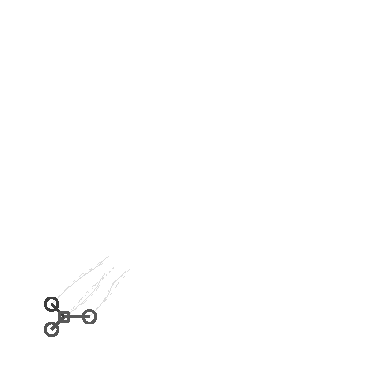
\includegraphics[scale=0.6]{figures/holonomic_0_tikz_gray.pdf} &
			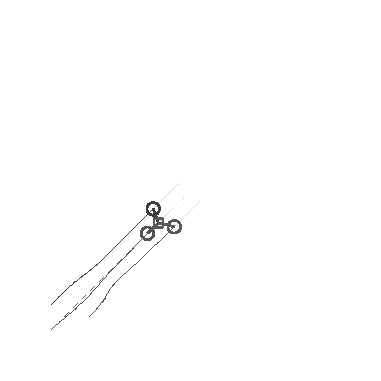
\includegraphics[scale=0.6]{figures/holonomic_1_tikz_gray.pdf} &
			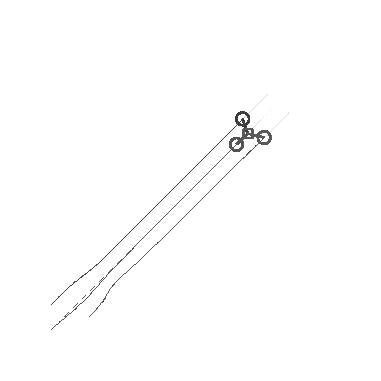
\includegraphics[scale=0.6]{figures/holonomic_2_tikz_gray.pdf} &
			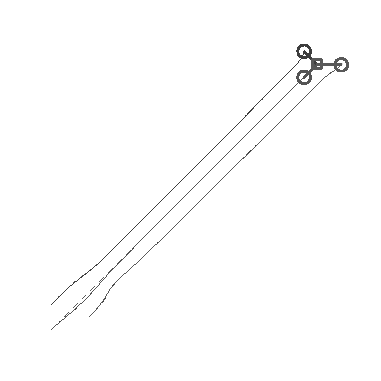
\includegraphics[scale=0.6]{figures/holonomic_3_tikz_gray.pdf} \\
		\hline
	\end{tabular}
	\caption{Motion trajectories for the payload and holonomic vehicles within the multi-agent system. The dotted lines represent payload trajectory. The gray lines indicate the computed trajectories to follow. The black lines represent the covered paths.}
	\label{trajectories}
\end{figure*}
From this least squares problem, it can be seen the consensus variables $\cz_{ij}$ are pushed between the \textit{expected} $\cx_{ij}$ variables and the \textit{actual} $\cx_j$ variables, acting as a balance between them. In the first ADMM step (Step 7), the reverse occurs in that $\cx_{ij}$ and $\cx_j$ are pushed towards the previous \textit{compromise} $\cz_{ij}$ variables. Thus, over MPC (and hence, ADMM) iterations, a consensus is achieved between $\cx_{ij}$ and $\cx_j$, resulting the problem dynamics being satisfied.

\section{Simulation results}
The DMPC strategy proposed in Algorithm~\ref{alg:dmpc} is numerically validated for the multi-agent system with parameters $m_0$= 5kg, $m_i$=2kg, $c_i$=20Ns/m and $K_i$=50N/m.
The velocities and accelerations of the vehicles are enforced to start from 0$m/s$ and 0$m/s^2$ respectively. The initial positions have been chosen such that the payload starts from a balanced state. The vehicle and payload trajectories are parameterized as B-splines with cubic basis functions having 10 knot intervals. This parameterization avoids conservatism. The time horizon is $T$ = 5s, and each DMPC update happens every $\Delta T$ = 0.1s. The ADMM penalty parameter is $\rho$ = 0.5. The optimization problem in step 7 of Algorithm~\ref{alg:dmpc} is solved using the interior point solver IPOPT \cite{c17}, for which the exact Jacobians and Hessians are provided by CasADi \cite{c18}. The initial conditions for each DMPC update in the simulations are obtained following the assumption of perfect tracking of trajectories calculated in the previous DMPC update by the vehicles.
\indent
\subsection{Payload transportation in an obstacle-free environment}
The motion trajectories of the vehicles and payload upon implementation of Algorithm~\ref{alg:dmpc} to control the multi-agent system are shown in Figure \ref{trajectories}. The darker lines represent trajectories that have been traversed by the vehicles and payload, and the lighter lines represent future trajectories. The corresponding velocity trajectories tracked by the vehicles are shown in Figure \ref{velocities}.
\begin{figure}[H]
	\centering
	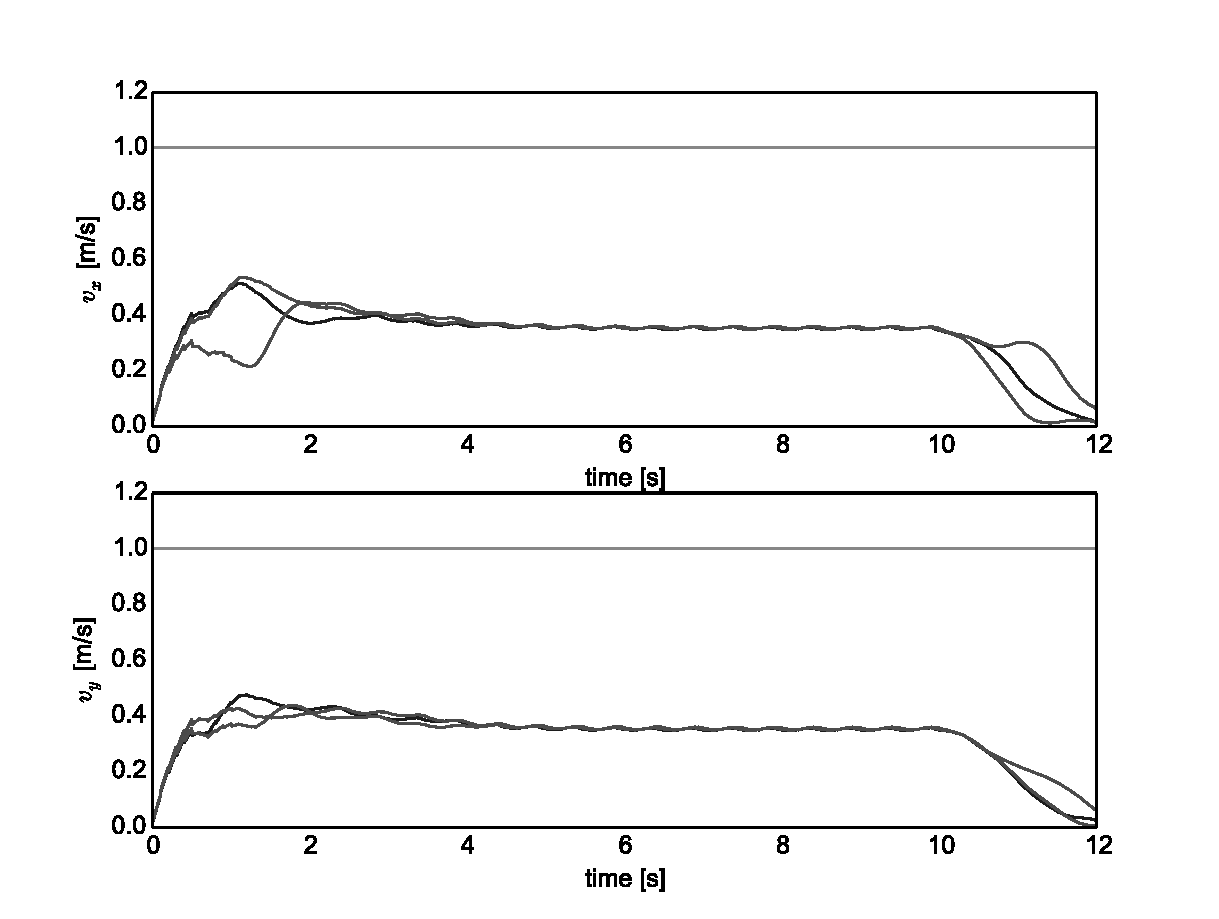
\includegraphics[scale=0.40]{figures/velocities_gray.pdf}
	\caption{Velocity trajectories of the vehicles. Dark line at 1 m/s indicates constraint.}
	\label{velocities}
\end{figure}
Since consensus constraints such as $\cx_{i0} = \cx_{j0}$ are not imposed, the payload positions are free to evolve according to the local dynamics of each vehicle. However, the complete multi-agent system dynamics are satisfied only if the local payload position copies converge towards each other. Hence, convergence of local payload positions towards each other over successive ADMM iterations is an indicator for dynamics satisfaction. This convergence is monitored by using distance metrics between the payload trajectory coefficients $\cx_{10}$, $\cx_{20}$ and $\cx_{30}$,  calculating a measure of dynamics error $\epsilon_0$ as:
\begin{equation}
\epsilon_0 = \mathlarger{\sum_{i=1}^{3}} \mathlarger{\sum_{j \neq i}} \mathlarger{\langle} \cx_{i0} - \cx_{j0},\cx_{i0} - \cx_{j0} \mathlarger{\rangle}
\end{equation}
For the trajectories shown in Figure \ref{trajectories}, the corresponding $\epsilon_{0}$ is shown in Figure \ref{error}.
\begin{figure}[H]
	\centering
	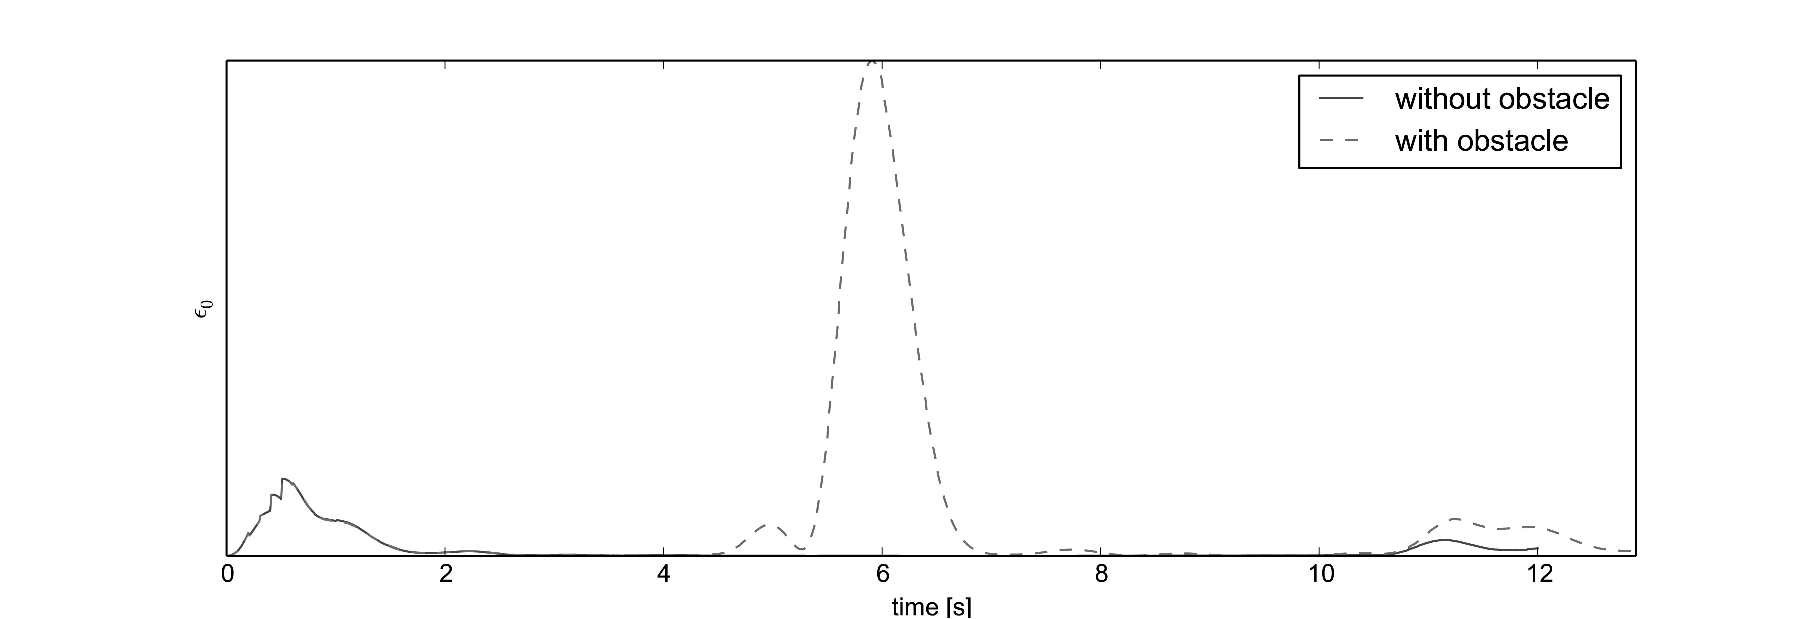
\includegraphics[scale=0.3]{figures/epsilons.pdf}
	\caption{Error in system dynamics.}
	\label{error}
\end{figure}
\indent
\begin{figure*}[t]
	\centering
	\vspace{-5pt}
	\setlength{\tabcolsep}{0.1em}
	\begin{tabular}[t]{|c|c|c|c|}
			\hline
				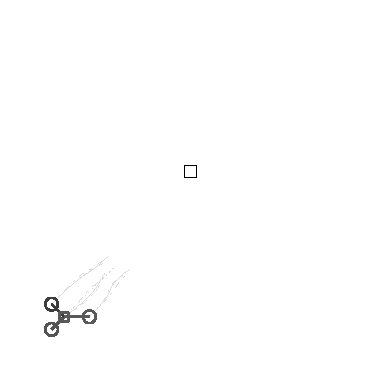
\includegraphics[scale=0.6]{figures/obstacle_0_tikz_gray.pdf} &
				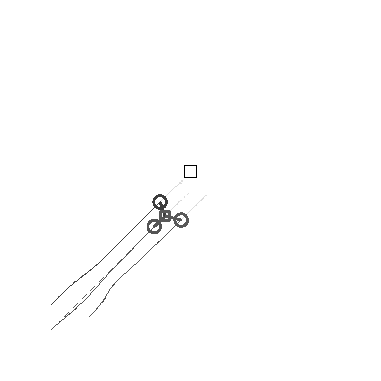
\includegraphics[scale=0.6]{figures/obstacle_1_tikz_gray.pdf} &
				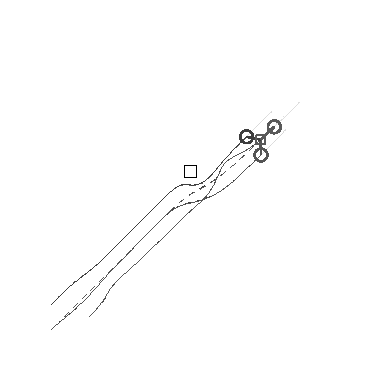
\includegraphics[scale=0.6]{figures/obstacle_2_tikz_gray.pdf} &
				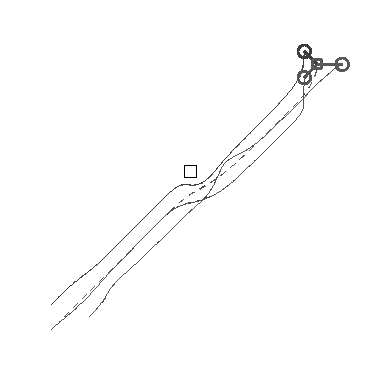
\includegraphics[scale=0.6]{figures/obstacle_3_tikz_gray.pdf} \\
			\hline
		\end{tabular}
	\caption{Motion trajectories of the vehicles and payload in the presence of a stationary obstacle.}
	\label{obstacle}
\end{figure*}
Since all vehicles start with the same initial value of the payload position, the coefficients match resulting in $\epsilon_0$=0. However, the local payload copies diverge from each other during the initial few DMPC iterations, and before halt of the payload. This is because each vehicle $i$ is agnostic of each other vehicle $j$'s force limits. At the start, the vehicle $i$ requests a trajectory $\cx_{ij}$ of vehicle $j$ which results in an immediate pull of the payload with a high force. Towards the end, the opposite occurs with each vehicle $i$ requesting a $\cx_{ij}$ pulling the payload to an immediate halt. However, vehicle $j$ can
 realistically only provide a trajectory $\cx_j$ while respecting its own constraints. This trajectory is different from the requested $\cx_{ij}$, resulting in a loss of consensus. The local payload dynamics thus evolve with a different set of inputs on each vehicle, increasing the value of $\epsilon_0$. This disagreement is however penalized through the consensus variables $\cz_{ij}$, and dual variables $\lambda_{ij}$ and $\mu_{ij}$. The penalization results in the vehicles achieving consensus on the payload position over successive DMPC iterations, reducing the value of $\epsilon_0$. Hence, it is concluded that the dynamics of the complete multi-agent system are satisfied. The number of iterations after which consensus is achieved can be reduced by increasing the value of the ADMM penalty parameter $\rho$. However, this results in lower vehicle velocities indicating a loss in optimality with respect to payload transportation. \\
 The ability to achieve consensus can be seen as an indication of convergence of the real-time ADMM scheme. This is as expected, since the current optimization problem is convex. Non-holonomic vehicle models might introduce non-convexity into the problem, resulting in a loss of convergence. Further investigation into these properties is currently being performed, in addition to robustness with respect to noises, parameter variabilities and communication delays.
 \indent
 \subsection{Payload transportation with obstacle avoidance}
Static obstacle avoidance behavior is obtained by adding additional spline variables representing separating hyperplane coefficients, as discussed in \cite{c15}. Each vehicle $i$ is assigned a set of these variables $a_i(t)$ and $b_i(t)$, for which the separating hyperplane constraints are defined. These constraints make sure that the trajectories $x_i(t)$, $x_{i0}(t)$ and $x_{ij}(t)$ lie on one side of the separating hyperplane parameterized by $a_i(t)$ and $b_i(t)$, and the obstacle lies on the other side of the hyperplane. The trajectories generated with this behavior is shown in Figure \ref{obstacle}. Near the obstacle, there is a loss of consensus between $\cx_{ij}$ and $\cx_{j}$, which is regained over successive ADMM iterations. Like before, the rate at which the consensus is regained can be controlled by tuning the ADMM penalty parameter $\rho$. 
\indent

 \section{Conclusion and future work}
This paper presents an algorithm to solve the multi-vehicle payload transportation problem in a Distributed Model Predictive Control (DMPC) framework. The optimization problem underlying the control problem is decoupled over the multiple vehicles based on the Alternating Direction Method of Multipliers (ADMM). A novel variable copying scheme is adopted, which results in a decentralized consensus formulation for a dynamically coupled system. Results based on numerical simulations are observed, and consensus on payload position is noted leading to the conclusion that the coupled dynamics are satisfied over successive iterations of the DMPC algorithm. It is noted that algorithms developed along the same lines can be applied to systems with $N\geq$2 vehicles. Future work includes modifying the algorithm to include dynamics considering free length of the flexible elements, which makes practical validation with real-life holonomic vehicles feasible. Further modifications can be done to the algorithm to analyze the effects of additional constraints imposing consensus on local payload copies and separating hyperplane variables on dynamic behavior.

%\begin{thebibliography}{99}
\bibliography{references_ecc}
%\end{thebibliography}%

\end{document}
